\section{Filtro 1: Blur}

\subsection{Cambios}
Para el recuperatorio decidimos hacer cambios en el codigo.

La lista de cambios esta a continuacion, con la aclaracacion de por que se hicieron los mismos:
\noindent
\begin{itemize}
\item Se remplazaron las operaciones que realizaban las copias por operaciones de SIMD para aumentar la velocidad a la que se copian los pixeles, tambien se modifico el codigo el cual antes copiaba las dos filas de pixeles superiores para que solo copie una (Swapeando los punteros de R13 con R12 y luego solo copiando en R13 los datos de la fila de pixeles del medio).
\end{itemize}

\subsection{Explicacion}

El filtro $blur$ consiste en para cada pixel (exceptuando los ubicados en el borde), tomar sus 8 vecinos y hacer un promedio de cada uno de sus componentes \texttt{R}, \texttt{G} y \texttt{B} entre los 9 pixeles, este nuevo valor reemplaza los que teniamos en el pixel actual. El promedio debe ser calculado respecto a los datos originales, es decir, que si al procesar un pixel y alguno de los vecinos ya fue procesado, debemos utilizar los datos del mismo antes de la modificacion. Nuestro algoritmo se basara en el implementado por la catedra en $C$ pero aprovechando de las operaciones vectoriales de SIMD para mejorar su performance tratando de trabajar con la mayor cantidad de datos al mismo tiempo.

\subsection{Implementacion 1}
La primera implementacion nos pide trabajar de a 1 pixel por iteracion.

Los pixeles estan compuestos por 4 bytes: \texttt{A R G B}, esto nos permite cargar 4 pixeles en un registro \texttt{XMM}, como nosotros necesitamos 9 pixeles, ubicados de a 3 en 3 filas diferentes vamos a precisar 3 registros \texttt{XMM} para cargarlos (Para esto usamos los registros \texttt{XMM0}, \texttt{XMM2} y \texttt{XMM4}). Ademas se utilizaron los siguientes 6 registro de proposito general: \\

\noindent
\begin{itemize}
\item \texttt{RDI} que lo usamos para iterar sobre el eje \texttt{X}
\item \texttt{R9} que lo usamos para iterar sobre \texttt{Y}
\item \texttt{R12} que es un puntero a la copia de la fila superior
\item \texttt{R13} que es un puntero a la copia de la fila actual
\item \texttt{R8} es un puntero a la fila inferior
\item \texttt{R10} es un puntero a la fila actual de la imagen (fila que estoy modificando)
\end{itemize}

Esto se puede visualizar en el siguiente grafico:

\begin{figure}[h!]
	\centering
	\includegraphics[scale=0.5]{images/BlurASM1_0}
\end{figure}

Donde \texttt{P} es el pixel a procesar.

Antes de comenzar el ciclo incicializamos \texttt{RDI} en 0, \texttt{R9} en 2, movimos \texttt{R8} a \texttt{R10}, aumentamos \texttt{R8} en una fila y posicionamos el puntero a la imagen en memoria en la segunda fila de pixeles.

Al principio de cada ciclo copiamos en los registros los 3 grupos de pixeles y quedan de la siguiente manera:\\

\noindent
\texttt{XMM0 $\gets$ [R12 + RDI] = - $\vert$ p2 $\vert$ p1 $\vert$ p0}\\
\texttt{XMM1 $\gets$ [R13 + RDI] = - $\vert$ p5 $\vert$ p4 $\vert$ p3}\\
\texttt{XMM2 $\gets$ $\ $[R8  + RDI] = - $\vert$ p8 $\vert$ p7 $\vert$ p6}\\

Despues desempaquetamos los pixeles de $byte$ a $word$ para poder sumar los 9 pixeles sin saturacion, hicimos una copia de cada uno para poder desempaquetar la parte inferior en un registro y la superior en otro (\texttt{XMM1 = XMM0}, \texttt{XMM3 = XMM2}, \texttt{XMM5 = XMM4}) y ademas llenamos un registro (\texttt{XMM12}) con ceros para expandir cada una de las componentes sin alterar el numero original.
Una vez desempaquetados nos quedan los registros con los siguientes valores:\\

\noindent
\texttt{XMM0 $\gets$ p1 $\vert$ p0} \\
\texttt{XMM1 $\gets$ - $\ \vert$ p2} \\
\texttt{XMM2 $\gets$ p4 $\vert$ p3} \\
\texttt{XMM3 $\gets$ - $\ \vert$ p5} \\ 
\texttt{XMM4 $\gets$ p7 $\vert$ p6} \\
\texttt{XMM5 $\gets$ - $\ \vert$ p8} \\
\\
Luego sumamos los registros e hicimos la division. \\

Sumando \texttt{XMM0}, \texttt{XMM2} y \texttt{XMM3} en \texttt{XMM15}: \\
	\texttt{XMM15 $\gets$ p1 + p4 + p7 $\vert$ p0 + p3 + p6}	\\

Sumando \texttt{XMM1}, \texttt{XMM3} y \texttt{XMM4} en \texttt{XMM14}	\\
	\texttt{XMM14 $\gets$ - $\vert$ p2 + p5 + p8} \\

Luego hicimos una copia de \texttt{XMM15} en \texttt{XMM13} y la shifteamos 8 bytes a la derecha \\
	\texttt{XMM13 $\gets$ - $\vert$ p1 + p4 + p7} \\

Por ultimo sumamos \texttt{XMM15}, \texttt{XMM14} y \texttt{XMM13} en \texttt{XMM15} \\
	\texttt{XMM15 $\gets$ - $\vert$ p0 + p1 + p2 + p3 + p4 + p5 + p6 + p7 + p8} \\

Para hacer la division optamos por multiplicar por $(2^{16} / 9) + 1$ y luego shiftear 16 bits a la derecha cada componente. Para eso tengo el valor por el cual voy a multiplicar en memoria precalculado, al principio del programa decidimos guardarlo en \texttt{XMM11}.
Luego, hicimos una copia de \texttt{XMM15} en \texttt{XMM14} y multiplicamos por \texttt{XMM12} guardando la parte superior de la mutiplicacion en \texttt{XMM15} y la inferior en \texttt{XMM14}. Luego empaquetamos los dos valores juntos como doubleword y los guardamos en \texttt{XMM14} y shifteamos 16 bits a la derecha.
Por ultimo empaquetamos los valores obtenidos a words y luego a bytes, posteriorment los guardamos en la posicion de memoria del pixel actual.

Aumentamos en 4 el iterador en \texttt{X} y comparamos con el tamaño en bytes de una linea de pixeles, si es menor iteramos nuevamente. En caso de que fuese mayor o igual, copiamos cambiamos los punteros de \texttt{R12} y \texttt{R13} y luego copiamos en R13 los pixeles de la siguiente fila (las cuales seran necesarias para poder operar la siguiente fila).

Para terminar copiamos \texttt{R8} en \texttt{R10}, movemos \texttt{R8} una fila de pixeles, reseteamos el iterador X \texttt{RDI}, incrementamos el iterador en Y \texttt{R9} y si el iterador de Y es menos a la altura de la imagen iteramos nuevamente.

\subsection{Implementacion 2}
Para la segunda implementacion se nos pidio trabajar de a 4 pixeles por iteracion.

Para eso calculamos primero los pixeles \texttt{P0} y \texttt{P1}, y despues el \texttt{P2} y \texttt{P3} tratando de minimizar la cantidad de accesos a memoria. \\

\begin{figure}[h!]
	\centering
	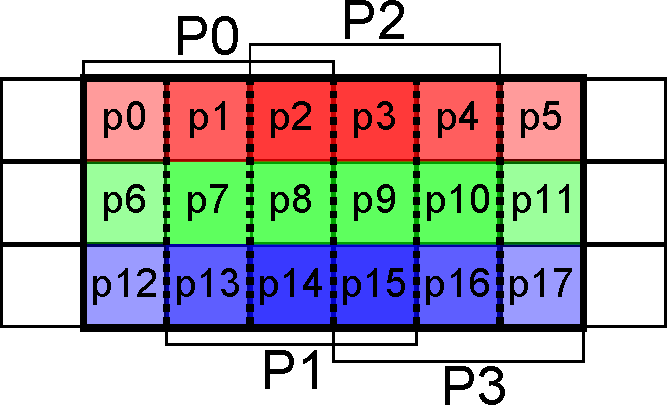
\includegraphics[scale=0.5]{images/BlurASM2_1}
\end{figure}

Para hacer los calculos tomamos 6 set de 4 pixeles que nos permiten sumar en un solo registro 2 pixeles al mismo tiempo usando solo sumas, cada set ira adentro de un registro \texttt{XMM}. Ademas necesitamos 6 registros \texttt{XMM} mas para poder desempaquetar los bytes a words, y asi no tener saturacion. \\

\newpage
Al igual que la primer implementacion, necesitaremos los mismos 6 registros de proposito general. \\

\begin{figure}[h!]
	\centering
	\includegraphics[scale=0.5]{images/BlurASM2_0}
\end{figure}

Antes de comenzar el ciclo incicializamos \texttt{RDI} en 0, \texttt{R9} en 2, movimos \texttt{R8} a \texttt{R10}, aumentamos \texttt{R8} en una fila y posicionamos el puntero a la imagen en memoria en la segunda fila de pixeles.

Luego cargamos los 6 pixeles a sus respectivos registros:\\

\noindent
\texttt{XMM0 $\ \gets$ p3 $\ \vert$ p2 $\ \vert$ p1 $\ \vert$ p0} \\
\texttt{XMM2 $\ \gets$ p4 $\ \vert$ p3 $\ \vert$ p2 $\ \vert$ p1} \\
\texttt{XMM4 $\ \gets$ p9 $\ \vert$ p8 $\ \vert$ p7 $\ \vert$ p6} \\
\texttt{XMM6 $\ \gets$ p10 $\vert$ p9 $\ \vert$ p8 $\ \vert$ p7} \\
\texttt{XMM8 $\ \gets$ p15 $\vert$ p14 $\vert$ p13 $\vert$ p12} \\
\texttt{XMM10 $\gets$ p16 $\vert$ p15 $\vert$ p14 $\vert$ p13} \\

De la misma forma que en la primer implementacion desempaquetamos los registros haciendo una copia y desempaquetando la parte superior en el registro original y la inferior en la copia. Para desenpaquetar usamos un registro con ceros (\texttt{XMM15}) \\

\noindent
\texttt{XMM0 $\ \gets$ p1 $\ \vert$ p0} \\
\texttt{XMM1 $\ \gets$ p3 $\ \vert$ p2} \\
\texttt{XMM2 $\ \gets$ p2 $\ \vert$ p1} \\
\texttt{XMM3 $\ \gets$ p4 $\ \vert$ p3} \\ 
\texttt{XMM4 $\ \gets$ p7 $\ \vert$ p6} \\
\texttt{XMM5 $\ \gets$ p9 $\ \vert$ p8} \\
\texttt{XMM6 $\ \gets$ p8 $\ \vert$ p7} \\
\texttt{XMM7 $\ \gets$ p10 $\ \vert$ p9} \\
\texttt{XMM8 $\ \gets$ p13 $\ \vert$ p12} \\
\texttt{XMM9 $\ \gets$ p15 $\ \vert$ p14} \\ 
\texttt{XMM10 $\gets$ p14 $\ \vert$ p13} \\
\texttt{XMM11 $\gets$ p16 $\ \vert$ p15} \\

Con todos los registros cargados, procedimos a sumar cada uno de ellos con XMM15, el resutlado final fue el siguiente:\\

\noindent
\texttt{XMM15 $\gets$ p1 + p2 + p3 + p7 + p8 + p9 + p13 + p14 + p15 $\vert$ p0 + p1 + p2 + p6 + p7 + p8 + p12 + p13 + p14}\\

Como podemos apreciar, el mismo responde al grafico presentado anteriormente, particularmente a los pixeles \texttt{P0} y \texttt{P1}. Luego hicimos la division de cada pixel de la misma manera que en la primer implementacion, antes de dividir preservamos una copia de \texttt{XMM15} en \texttt{XMM9}, dividimos por 9, shifteamos 8 bytes y dividimos nuevamente. Finalmente movimos los pixeles procesados a \texttt{P0} y \texttt{P1} a la memoria en la posicion correcta. Despues hubo que procesar los pixeles \texttt{P2} y \texttt{P3}, para hacer esto movimos 3 grupos mas de pixeles de la memoria hacia los registros. En esta etapa tenemos:

\noindent
\texttt{XMM0 $\gets$ p5 $\ \vert$ p4 $\ \vert$ p3 $\ \vert$ p2}\\
\texttt{XMM4 $\gets$ p11 $\vert$ p10 $\vert$ p9 $\ \vert$ p8}\\
\texttt{XMM8 $\gets$ p17 $\vert$ p16 $\vert$ p15 $\vert$ p14}\\

Luego hicimos copias en \texttt{XMM1}, \texttt{XMM5} y \texttt{XMM9} y desempaquetamos de byte a word:\\

\noindent
\texttt{XMM0 $\gets$ p3 $\ \vert$ p2}\\
\texttt{XMM1 $\gets$ p5 $\ \vert$ p4}\\
\texttt{XMM4 $\gets$ p9 $\ \vert$ p8}\\
\texttt{XMM5 $\gets$ p11 $\vert$ p10}\\
\texttt{XMM8 $\gets$ p15 $\vert$ p14}\\
\texttt{XMM9 $\gets$ p17 $\vert$ p16}\\

Nuevamente sumamos los registros de la misma forma que antes, es decir, uno a uno con \texttt{XMM15}, el resultado final es:\\

\noindent
\texttt{XMM15 $\gets$ p3 + p4 + p5 + p9 + p10 + p11 + p15 + p16 + p17 $\vert$ p2 + p3 + p4 + p8 + p9 + p10 + p14 + p15 + p16}

Como podemos apreciar, en este caso las cuentas tambien responden a lo presentado en los graficos, en este caso a los pixeles \texttt{P2} y \texttt{P3}. De la misma forma que antes hacemos las divisiones apropiadas, y guardamos los pixeles procesdos en memoria.

Una vez terminado el procesamiento de pixeles, comparamo el iterador con la cantidad de pixeles en una fila y repetimos hasta llegar hasta los ultimos 16 bytes de la fila, estos ultimos 16 bytes los cargamos en solo 3 registros \texttt{XMM} y los procesamos al igual que la primera parte del ciclo para asegurarme de no pasarnos. Al final del ciclo hacemos las copias pertinentes, incrementamos el iterador de filas y revisamos si llegamos al final. \\

\subsection{Resultados}
Para la experimentacion vamos a correr las 3 implementaciones (La version de C compilada con optimizaciones de nivel 3) para poder comparar la performance, vamos a usar la imagen de $lena$ brindada por la catedra (Resolucion 160x160). Se ejecutara cada implementacion del algoritmo 100 veces y luego se calculara el tiempo (Usando el time stamp counter del procesador y la funcion de C brindada por la catedra) minimo, maximo y promedio (Sumando todos los tiempos tomados y diviendo por el la cantidad de iteraciones). A continuacion graficamos los tiempos en un grafico de barras que esta a continuacion:

\begin{figure}[h!]
	\centering
	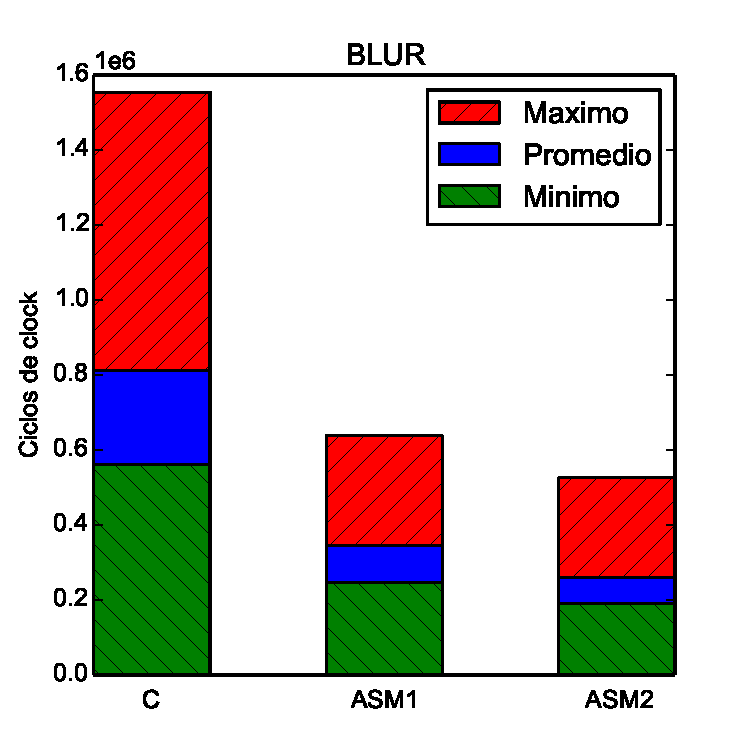
\includegraphics[scale=0.45]{images/blur_comparation}
\end{figure}

Con esto podemos ver que la implementacion ASM2 es un poco mas rapida que las otras implementaciones.

Revisando el codigo podemos ver que el tamaño de la imagen solo deberia modificar cantidad de pixeles a procesar aumentando el tiempo de ejecucion solo por que se necesita hacer mas iteraciones, tambien podemos ver que el algoritmo es independiente del color de los pixeles a procesar.

Para la reentrega se hicieron algunos cambios en el codigo que se supone que deberian mejorar la performance (Ver lista de cambios), decidimos correr el test explicado anteriormente el codigo nuevo y el codigo viejo para comfirmar que los cambios propuestos cumplan con su objetivo. En el siguiente grafico graficaron los tiempos maximos, minimo y promedio de ejecucion de la implementaciones de ASM.

\begin{figure}[h!]
	\centering
	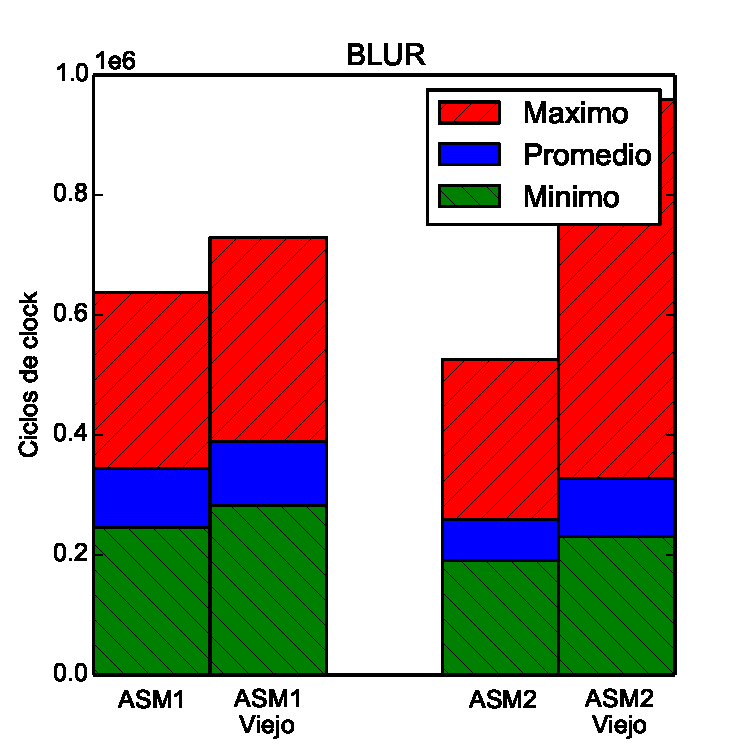
\includegraphics[scale=0.45]{images/blur_comparationOLD}
\end{figure}

\newpage

% Para la experimentacion vamos a correr las 3 implementaciones (La version de C compilada con optimizaciones de nivel 3) con la imagen de $lena$ brindada por la catedra (multiplos de 16x16, hasta 320x320). Cada tamaño se ejecuta 100 veces, despues se saca un promedio y se lo grafica junto con el maximo y el minimo. La metodologia adoptada para evaluar la eficacia de las implementaciones es tomar la cantidad de ciclos que tarda en correr cada una de las implementaciones, esto lo hacemos mediante la libreria \texttt{rdtsc.h}, las pruebas van a ser ejecutadas en un \texttt{Intel Core i7 4700MQ}. Estas condiciones de prueba se mantendran durante el resto del informe y para todos los filtros.

% \begin{figure}[h!]
% 	\centering
% 	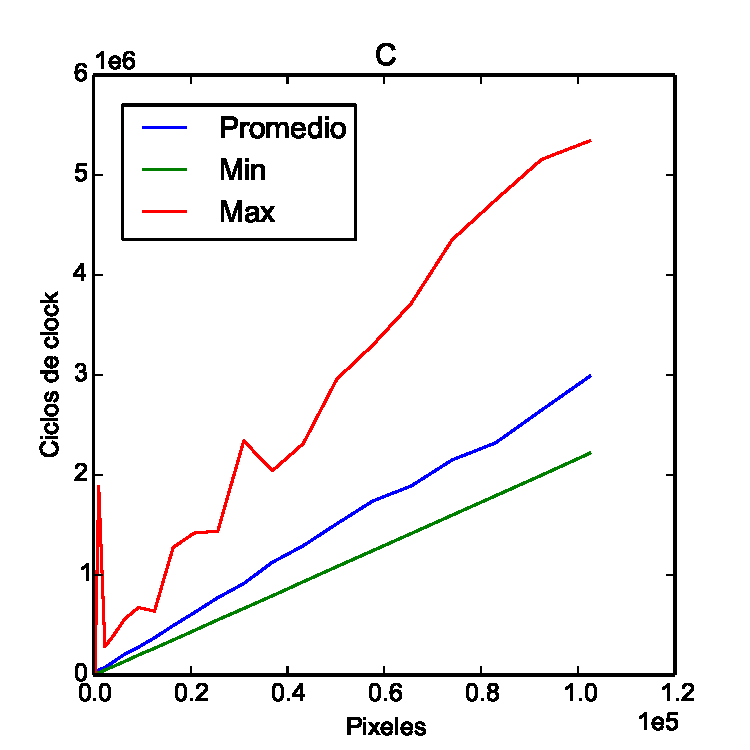
\includegraphics[scale=0.45]{images/c_blur}
% 	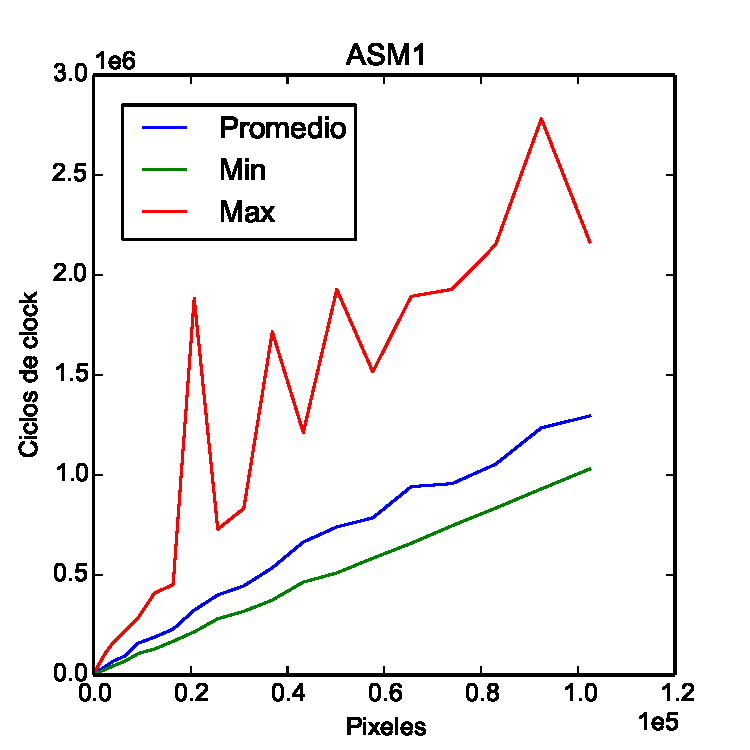
\includegraphics[scale=0.45]{images/asm1_blur}
% 	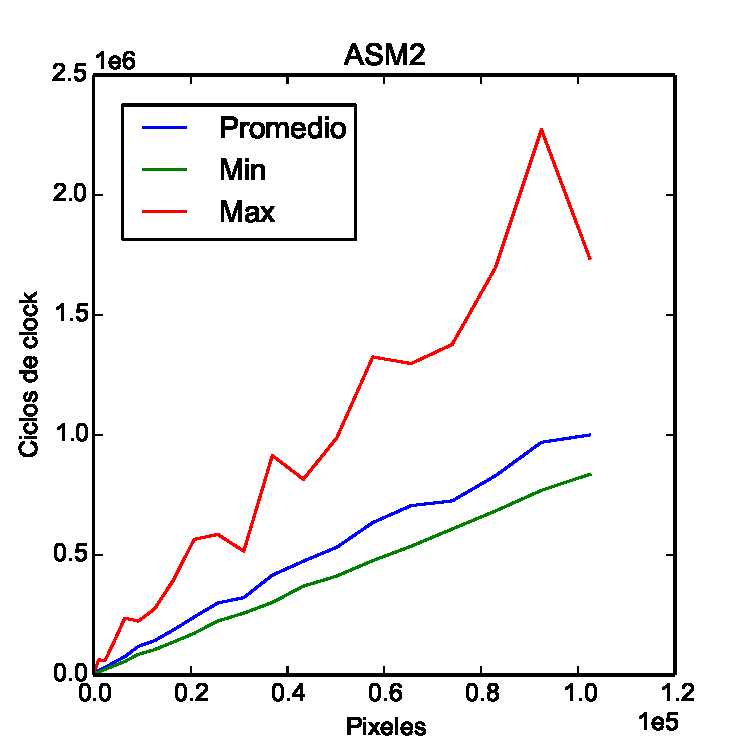
\includegraphics[scale=0.45]{images/asm2_blur}
% \end{figure}

% Ahora graficamos los 3 valores promedios de $blur$ para ver cual de ellos es el mas rapido en general. Para ver mejor la diferencia entre ASM1 y ASM2 los graficamos aparte.

% \begin{figure}[h!]
% 	\centering
% 	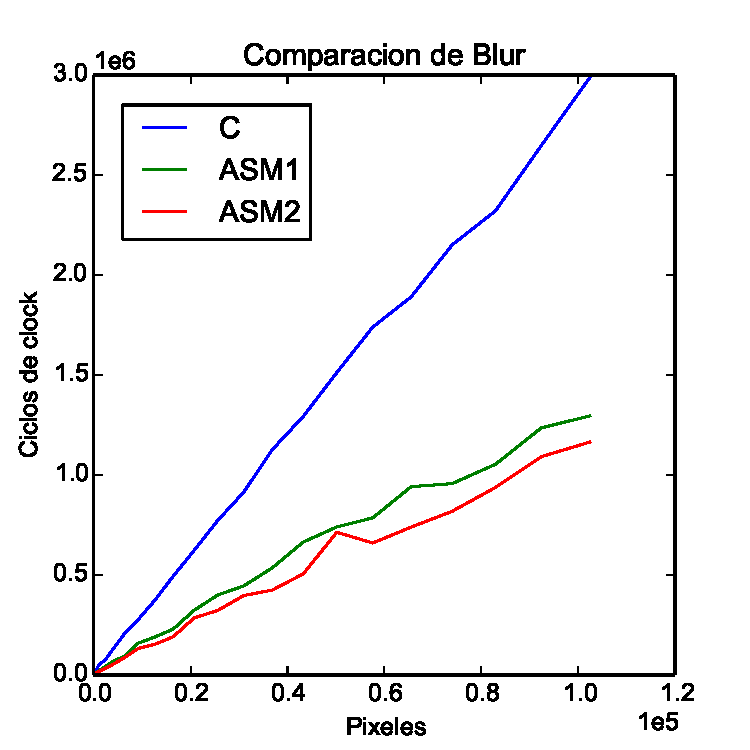
\includegraphics[scale=0.5]{images/c_asm1_asm2_blur_comp}
% 	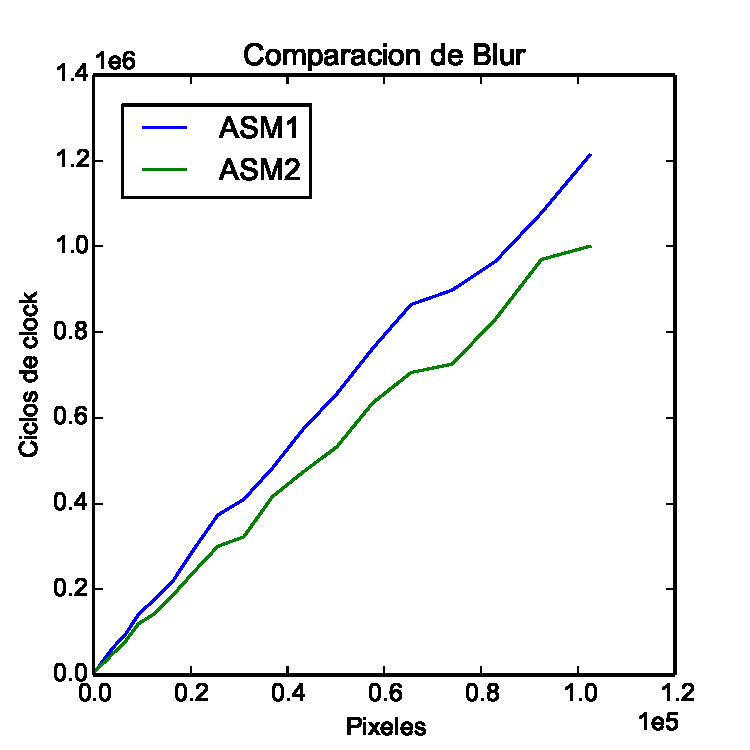
\includegraphics[scale=0.5]{images/asm1_asm2_blur_comp}
% \end{figure}

% Este grafico nos muestra que el codigo de ASM2 pareceria ser el mas rapido. Antes de confirmar esto queremos ver que no haya ningun tipo de factor en la imagen que influya en el tiempo de ejecucion que no sea el tamaño. \\

% Tanto en el codigo de C como en el ASM1 y ASM2 no poseen ninguna operacion que dependa de los pixeles a procesar, para probar que esto es realmente asi en la practica decidimos correr los test al igual que al principio pero esta vez usando la imagen de $lena$, $colores$ y 3 imagenes mas completamente rojas, azules y verdes.\\

% \begin{figure}[h!]
% 	\centering
% 	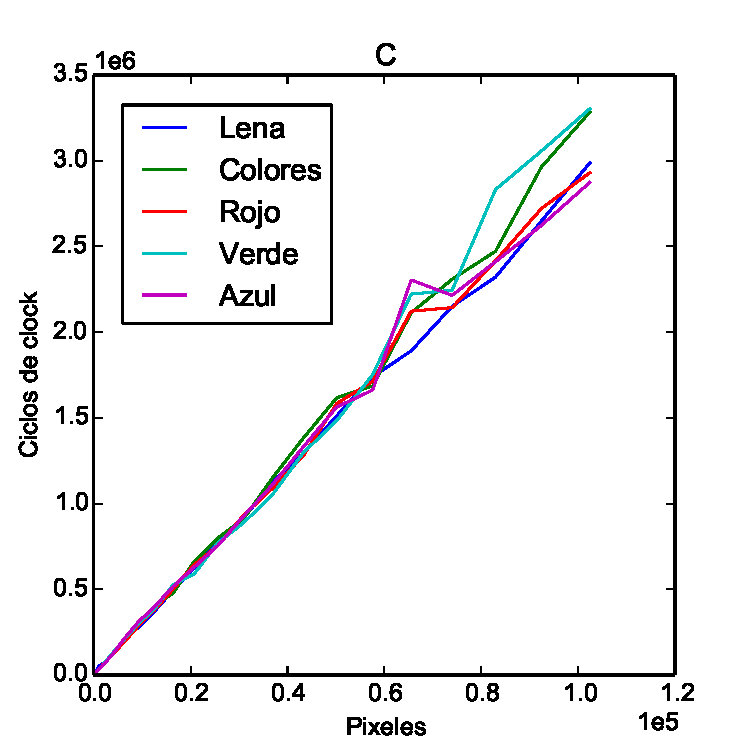
\includegraphics[scale=0.45]{images/c_blur_lena_colors}
% 	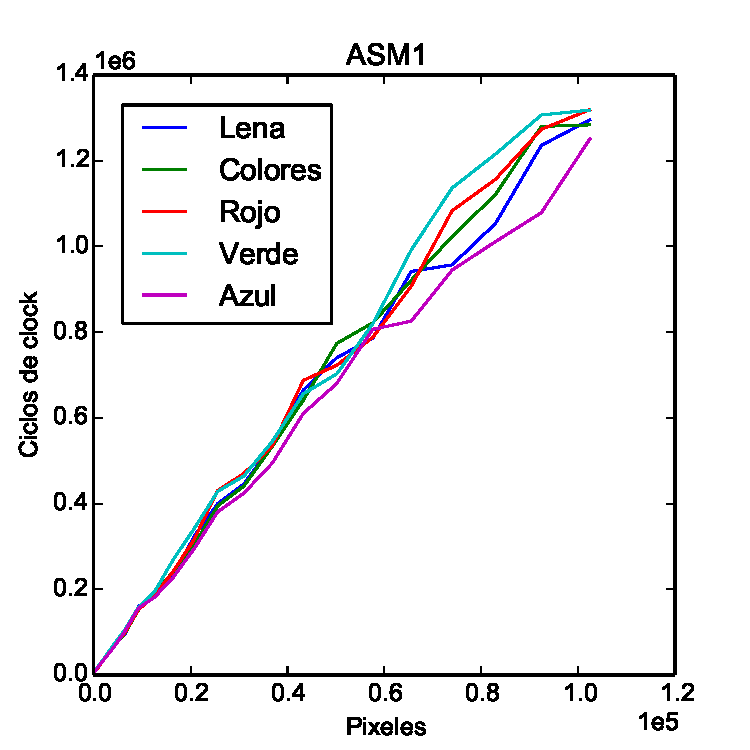
\includegraphics[scale=0.45]{images/asm1_blur_lena_colors}
% 	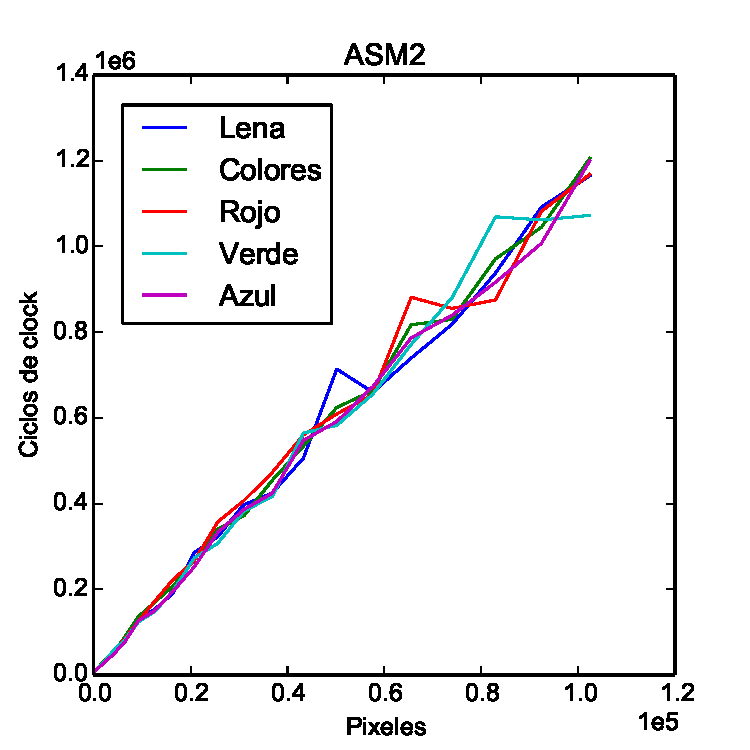
\includegraphics[scale=0.45]{images/asm2_blur_lena_colors}
% \end{figure}

\subsection{Conclusion}
Podemos concluir que en el caso de la utilizacion de instrucciones SIMD para la aplicacion del algoritmo de blur se puede ver que operar de a varios pixeles mejora un poco con respecto a operar de a un pixel pero al mismo tiempo tambien complica considerablemente el codigo que se debio implementar en nuestro caso.

Igual la simple implementacion de instrucciones SIMD comparandola con el codigo C compilado se puede notar una diferencia conciderable en cuanto a la cantidad de ciclos de reloj usados por el mismo.

% Luego de la experimentacion podemos concluir que ASM2 es el mas rapido en general. \\

% La imagen a procesar no afecta en nada el tiempo de ejecucion y el tamaño lo afecta solo por que se deben procesar mas pixeles. \\